\documentclass[11pt,
  paper=a4, 
  bibliography=totocnumbered,
	captions=tableheading,
	BCOR=10mm
]{scrreprt}

\usepackage[utf8]{inputenc}
 
 
\usepackage[onehalfspacing]{setspace}
\usepackage{csquotes} % Context sensitive quotation.
\usepackage{amsmath} % Standard math.
\usepackage{amsthm} % Math theorems.
\usepackage{amssymb} % More math symbols.
\theoremstyle{definition}
\newtheorem{definition}{Definition}[chapter]
 
\usepackage[section]{placeins} % Keep floats in the section they were defined in.
\usepackage{tabularx}
\usepackage{booktabs} % Scientific table styling.
\usepackage{floatrow} % Option for keeping floats in the place they were defined in the code.
\floatsetup[table]{style=plaintop}
\usepackage{hyperref} % Hyperlinks.
\usepackage[all]{nowidow} % Prevent widows and orphans.
\usepackage{xstring} % logic string operations
\usepackage[nopostdot, nonumberlist]{glossaries} % glossary for definitions and acronyms, without dot after entry and page reference 
\usepackage{bbm} % \mathbb on numerals.
\usepackage{csquotes}
\usepackage{mathtools}
\usepackage[ruled,vlined]{algorithm2e} %Pseudocode
\usepackage{scrhack} % Make warning go away.
\usepackage{graphicx}
\usepackage{subcaption} % Subfigures with subcaptions.
\usepackage{authoraftertitle} % Make author, etc., available after \maketitle
\usepackage{listofitems}
\usepackage{blindtext} % Placeholder text.
\usepackage[nopostdot, nonumberlist]{glossaries}
\makeglossaries % Generate the glossary

% \PassOptionsToPackage{obeyspaces}{url}%
\usepackage[backend=bibtex,% 
style=nature,% 
doi=true,isbn=false,url=false, eprint=false]{biblatex}
% \renewbibmacro*{url}{\printfield{urlraw}}

\addbibresource{bib/library.bib}

\DeclareStyleSourcemap{
  \maps[datatype=bibtex, overwrite=true]{
    \map{
      \step[fieldsource=url, final]
      \step[typesource=misc, typetarget=online]
    }
    \map{
      \step[typesource=misc, typetarget=patent, final]
      \step[fieldsource=institution, final]
      \step[fieldset=holder, origfieldval]
    }
  }
}

%\linespread{1.5} % set line spacing
 
\usepackage{listings} % rendering program code
\lstset{% general command to set parameter(s)
	basicstyle=\ttfamily\color{grey},          % print whole listing small
	keywordstyle=\color{black}\bfseries\underbar,
	% underlined bold black keywords
	identifierstyle=,           % nothing happens
	commentstyle=\color{white}, % white comments
	stringstyle=\ttfamily,      % typewriter type for strings
	showstringspaces=false}     % no special string spaces


\DeclareFontFamily{U}{mathx}{\hyphenchar\font45}
\DeclareFontShape{U}{mathx}{m}{n}{
      <5> <6> <7> <8> <9> <10>
      <10.95> <12> <14.4> <17.28> <20.74> <24.88>
      mathx10
      }{}
\DeclareSymbolFont{mathx}{U}{mathx}{m}{n}
\DeclareFontSubstitution{U}{mathx}{m}{n}
\DeclareMathSymbol{\bigtimes}{1}{mathx}{"91}

 

%%% Custom definitions %%%
% Shorthands
\newcommand{\ie}{i.\,e.~}
\newcommand{\eg}{e.\,g.~}
\newcommand{\ind}{\mathbbm{1}}
% Functions
\newcommand{\tpow}[1]{\cdot 10^{#1}}
\newcommand{\figref}[1]{(Figure \ref{#1})}
\newcommand{\figureref}[1]{Figure \ref{#1}}
\newcommand{\tabref}[1]{(Table \ref{#1})}
\newcommand{\tableref}[1]{Table \ref{#1}}
\newcommand{\secref}[1]{%
	\IfBeginWith{#1}{chap:}{%
		(cf. Chapter \ref{#1})}%
		{(cf. Section \ref{#1})}%
		}
\newcommand{\sectionref}[1]{%
	\IfBeginWith{#1}{chap:}{%
		Chapter \ref{#1}}%
		{\IfBeginWith{#1}{s}{%
			Section \ref{#1}}%
			{[\PackageError{sectionref}{Undefined option to sectionref: #1}{}]}}}
\newcommand{\chapref}[1]{(see chapter \ref{#1})}
\newcommand{\unit}[1]{\,\mathrm{#1}}
\newcommand{\unitfrac}[2]{\,\mathrm{\frac{#1}{#2}}}
\newcommand{\codeil}[1]{\lstinline{#1}}{} % wrapper for preventing syntax highlight error
\newcommand{\techil}[1]{\texttt{#1}}
\newcommand{\Set}[2]{%
  \{\, #1 \mid #2 \, \}%
}
% Line for signature.
\newcommand{\namesigdate}[1][5cm]{%
	\vspace{5cm}
	{\setlength{\parindent}{0cm}
	\begin{minipage}{0.3\textwidth}
		\hrule 
		\vspace{0.5cm}
		{\small city, date}
	\end{minipage}
	 \hfill
	\begin{minipage}{0.3\textwidth}
		\hrule
		\vspace{0.5cm}
	    {\small signature}
	\end{minipage}
	}
}
% Automatically use the first sentence in a caption as the short caption.
\newcommand\slcaption[1]{\setsepchar{.}\readlist*\pdots{#1}\caption[{\pdots[1].}]{#1}}

% Variables. 
% Adapt if necessary, use to refer to figures and graphics.
\def \figwidth {0.9\linewidth}
\graphicspath{ {./graphics/figures/}{./graphics/figures/} } % Path to figures and images.


% Customizations of existing commands.
\renewcommand{\vec}[1]{\mathbf{#1}}
% Capitalized \autoref names.
\renewcommand*{\chapterautorefname}{Chapter}
\renewcommand*{\sectionautorefname}{Section}


% TODO Fill with your data.
\title{Image Segmentation}
\author{Sven Groen}

\begin{document}

\begin{titlepage}
	\begin{flushleft}
		Universität Osnabrück\\
		Fachbereich Humanwissenschaften\\
		Institute of Cognitive Science
	\end{flushleft}

	\vspace{2cm}
	\centering{
		Bachelorthesis - Expose \vspace{1cm}\\
		\textbf{\Large{\MyTitle}}
		\vspace{1cm}\\
		\begin{tabular}{c}
			\MyAuthor                          \\
			970219                            \\
			Bachelor's Program Cognitive Science 
		\end{tabular}}
	\vspace{1cm}

	\begin{tabular}{ll}
		First supervisor:  & Dr. Ulf Krumnack          \\
		                   & Institute of Cognitive Science            \\
		                   & Osnabrück                \\\\
		Second supervisor: & Manuel Kolmet         \\
		                   & IMANOX GmbH  \\
		                   & Berlin 
	\end{tabular}

\end{titlepage}


\pagenumbering{gobble}
\pagebreak


\tableofcontents


\chapter{Goal and background information}
\pagenumbering{arabic}

\section{Cooperation with Imanox}
This project is realized in cooperation with \href{https://www.imanox.de/}{Imanox} . 
Imanox is a Berlin-based Startup that developed a smart photo booth for expositions, events and promotions. 
This photo booth enables customers virtual product placements using augmented and mixed reality. 
Main features are hand-tracking, digital masks and changing virtual backgrounds.

\section{Virtual backgrounds}
Currently, the photo booth has a built in depth sensor that measures the distance of objects by casting illumination onto the scene and indirectly measuring the time it takes to travel back to the camera. 
The camera struggles with correctly predicting the depth in certain situations. 
Pixels are rendered as invalid and no depth information is provided. 
The reasons for this are numerous. 
Pixels might get under saturated (signal is not strong enough) or over saturated (signal is too strong). 
Other artifacts occur due to the geometry of the scene. 
The sensors of the camera might receive signals from multiple locations in the scene, leading to an ambiguous depth. 
Especially around the edges and borders of objects pixels contain mixed signals from fore-and background leading to blurred outlines.
In the current version of the photo booth alpha values (0 to 1) are calculated based on the data from the depth sensor. 
Objects in the foreground receive high alpha values and the background is considered to have an alpha value of 0, making it transparent. 
In this way the background can be virtually replaced without affecting the objects in the foreground. 
Due to the described inaccurate data that is given by the depth sensor the result is of low quality. 
The edges and borders of the objects or people in the scene are not sharp and often misclassified. 
Especially for small / thin objects, \eg hair, the camera hardly recognizes it and parts of the hair are therefore considered as background and are also replaced by the virtual background.
For more detailed information on this issue see \url{https://docs.microsoft.com/de-de/azure/Kinect-dk/depth-camera} \cite{Microsoft2019}.

\section{Goal of the thesis}
The goal of this bachelor thesis is to improve the quality of the semantic segmentation of the current Imanox photo booth using machine learning techniques.
The machine learning model will be one of the artificial neural network architectures (see Section~\ref{sec:related_work} for details).
This model will be altered and changed towards the needs of the project and will be trained with custom training data (see Section~\ref{sec:Method}).
It will be investigate whether high quality training data, which will be generated during the project, improves the visual result of the segmentation.
When looking at datasets that are very commonly used for semantic segmentation, such as COCO-dataset \cite{COCO2016}, one can notice that the outlines of the target labels are very rough and not detailed.
This might function as a bottleneck for a more detailed segmentation, one that would be able to grasp details such as hair.
The exact plan of how this detailed segmentation is achieved are not set yet.
Since the problem boils down to identifying the depth of objects in the scene, this thesis might also deal with the question of how additional depth information could be used to improve the result of models than usually just require two-dimensional images.
How this depth information is best gathered will be a subject of the thesis itself.
Lastly, it has been shown \cite{Nabavi2018, Pfeuffer2019} that using Convolutional Long-Short-Term-Memory (Conv-LSTM \cite{Shi2015}) layers help to improve the performance of already existing architectures.
The thesis will also explore whether adding these Conv-LSTM layers helps predicting the segmentation of future frames, given previous frames and whether the increase accuracy justifies the additional inference time.

\chapter{Segmentation}
\textcite{Szeliski2011} refers to image segmentation as "the task of finding groups of pixels that 'go together' " (p. 237).
In the following, semantic segmentation refers to a pixel-wise classification of an image \cite{Mittal2020}.
In the classical image classification tasks the task is to name the objects that can be seen in an image.
Semantic segmentation extends this problem further. 
Each pixel in an image is assigned to one category label given a set of categories.
However, individual instances of an object in one image are not differentiated.
When individual instances in an image should be recognized, object detection is necessary.
For single objects this would be a classification + localization task. 
Object detection is usually realized by framing the object with a box and assigning a category label to each box.
Lastly, there is instance segmentation. 
Instance segmentation extends the problem of object detection by a pixel-wise classification (similar to semantic segmentation) but with instances being differentiated \cite{Mittal2020}.
See \figref{fig:Computer_Vision_Tasks} for an overview of the described tasks.
Given the goal of this project, only semantic segmentation is necessary.
Detailed information about which objects are in the scene is not required.
\begin{figure}[H]
	\centering
	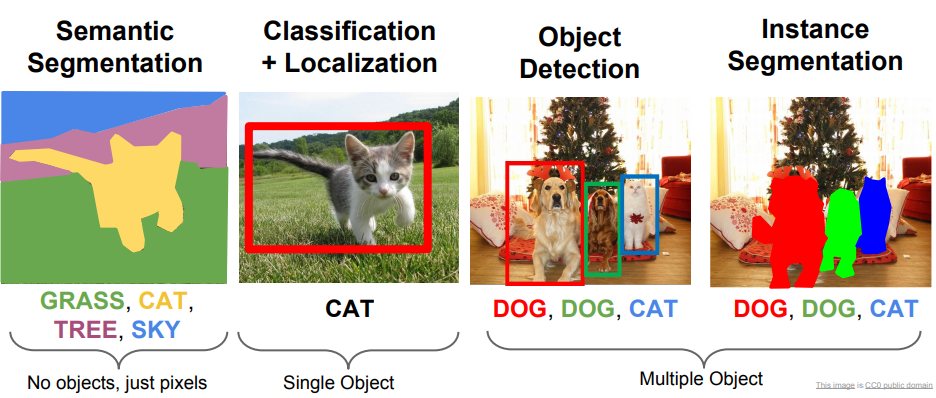
\includegraphics[width=\figwidth]{Computer_Vision_Tasks}
	\slcaption{
		Overview of Computer Vision Tasks. (\textcite{Fei-Fei2017}, Slide 17).
		\label{fig:Computer_Vision_Tasks}}
\end{figure}

\section{Related work}
\label{sec:related_work}

Segmenting an image into its individual parts is a classical problem of computer vision \cite{Szeliski2011}. 
Early approaches involve classical methods like threshold detection \cite{Smith1979}, while modern approaches like k-means clustering \cite{Dhanachandra2015} improved the results.
Deep learning architectures, especially convolutional neural networks (CNNs) \cite{Fukushima1980}, have lead to an improvement in performance whereas classical methods have seem to have reach a plateau \figref{fig:Object_Detect_impact_of_DL}.
\textcite{Shelhamer2017} have been the first to propose a CNN architecture where a pixel-wise supervised training was achieved. 
This was done by upsampling the class prediction layer to the input image size, leading to a pixel-wise classification, a Fully Convolutional Network (FCN).
Following papers proposed different architectures.
A "Deconvolutional Network" with special unpooling and deconvolution operations\cite{Noh2015}.
The SegNet model uses a similar Encoder-Decoder architecture by using pooling indices to upsample the image \cite{Badrinarayanan2017}.
ICNet \cite{Zhao2017} was able to perform semantic segmentation not only in real time, but also for high quality images (1024x2048 at 30 fps). 
This was achieved by using a cascade image input of different resolutions. 
The authors made use of the semantic information from the scaled down images and the details from the high resolution images.
Therefore, achieving a "trade-off between efficiency and accuracy" ( \cite{Zhao2017}, p.2).
Google's approach towards instance segmentation, called Deeplab, has evolved in recent years.
The first DeepLab version uses a combination of Deep CNNs with fully connected conditional random fields (CRFs) that tries to grasp the semantic context of the image \cite{Chen2018}.
The most recent approach, DeepLab V3+, has an Encoder-Decoder structure and was able to show "new state-of-the-art performance on PASCAL VOC 2012 and Cityscapes datasets." (\cite{Chen2018b}, p.14)
Moreover, the Google research team has shown that they are able to create an Encoder-Decoder architecture that is very light and fast.
This architecture is light enough to run at real time on modern smart phones \cite{Bazarevsky2018}.



\begin{figure}[H]
	\centering
	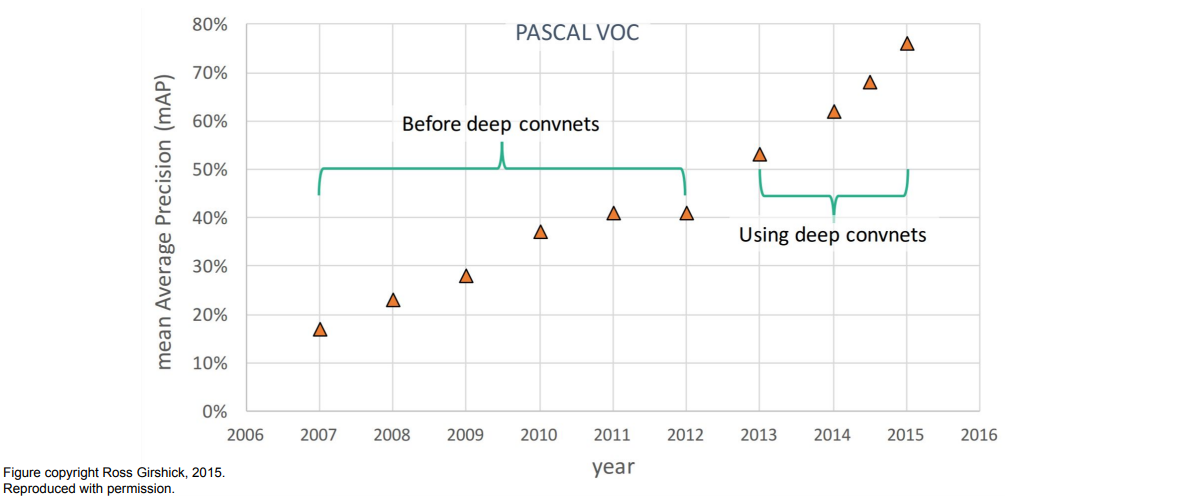
\includegraphics[width=\figwidth]{Object_Detect_impact_of_DL}
	\slcaption{
		Mean average precission (mAP) of object detection before and after using deep learning techniques. (\textcite{Fei-Fei2017}, Slide 54).
		\label{fig:Object_Detect_impact_of_DL}}
\end{figure}

Object detection algorithms also advanced using CNNs. 
The R-CNN architecture achieved a breakthrough by increasing the mAP "by more than 30\%
relative to the previous best result on VOC 2012" (\cite{Girshick2014}, p.1) by extracting region proposals which are then classified.
Reworking the architecture of the R-CNN model to increase the inference time, fast R-CNN \cite{Girshick2015} and faster R-CNN \cite{Ren2015} have been developed. 
While faster R-CNN achieved 5 fps \cite{Ren2015}, the first algorithms allowing real-time object detection have been the YOLO \cite{Redmon2016} and the SSD \cite{Liu2016} model.
In YOLO, the image is divided into a set of grid cells and for each grid cell, a set of 5 bounding boxes are proposed. 
Each bounding box returns a score that reflects if the box contains an object and in addition to that a class prediction for each box.
All of these bounding box informations plus its scores are fed into a Neural Network at once, instead of independently process the region proposals like in the R-CNN family, allowing YOLO object detection in real time \cite{Redmon2016}.

Combing the problem of semantic segmentation and object detection leads to instance segmentation.
The faster R-CNN structure has been extended to the mask R-CNN approach \cite{He2017}. 
The mask R-CNN model computes the bounding box coordinates, the class prediction and a binary segmentation mask in three different output branches \cite{Mittal2020}. 
The mask R-CNN model was able to extend the faster R-CNN architecture by adding a FCN branch while still running at 5 fps \cite{He2017}.
Real time instance segmentation was achieved by by YOLACT++. 
YOLACT++ breaks up instance segmentation into two simpler tasks that can be performed in parallel.
First, "prototype masks" are generated, second a set of "linear combination coefficients per instance" are predicted.
Lastly, the prototypes are combined in a linear manner using the predicted coefficients for each instance. 
This model is able to achieve real time ($>$30 fps) performance on only one powerful GPU \cite{Bolya2019}.

\section{Challenges}

There are several problems that have to be considered during the project:
\begin{enumerate}
	\item achieving a good tradeoff between high-quality results and low inference time (real-time performance)
	\item achieving invariance towards environmental disturbances (varying light conditions)
	\item working with high resolution images (4K)
\end{enumerate}

The ICNet and Deeplab V3+ has already shown that 1. and 3. are possible to solve by using information form low resolution input images.
2. is highly dependent on the training data. 
Hence, it has to be made sure that the training data contains possible environmental changes that might occur in real world scenarios.

\chapter{Method}
\label{sec:Method}

This thesis will investigate the current state of the art semantic segmentation concepts and evaluate which model is best suited, given the task description.
To achieve a high accuracy, training data will be generated.
Since the main task is to separate humans (and objects they might carry), training data will be generated using a green screen.
A green screen setup allows us to separate the background in a high quality manner using an alpha matting algorithm (\eg \cite{Gastal2010}).
The background in the training data can be virtually replaced with backgrounds that will be used in the photo booth in the final product.
This results in qualitatively high training data.
It is very likely, that the model will not be able to generalize very well beyond the given backgrounds, since the training data environment is very much controlled and fixed.
However, the final model does not have to generalize beyond the given scenario anyway. 

Given the architectures in Section~\ref{sec:related_work}, one can see that they share similar concepts (Encoder-Decoder architecture, Region proposals, etc.).
The project will most likely use either the YOLACT++ model, which is open source, delivers already high quality segmentation results and is able to run in real time or will adopt the Deeplab V3+ architecture, since it has already been shown that its complexity can be reduced heavily \cite{Bazarevsky2018}.

\chapter{Preliminary structure}

\begin{itemize}
	\item Declaration of Authorship
	\item Abstract
	\item Contents
	\item List of figures
	\item List of algorithms
	\item Introduction
	\begin{itemize}
		\item Motivation
		\item Goal of the thesis
	\end{itemize}
	\item Methods
	\begin{itemize}
		\item Model
		\item Training data
		\item Preprocessing
		\item Network training
	\end{itemize}
	\item Results and discussion
	\item Evalutation
	\item Conclusion
	\item Acknowledgements
	\item Bibliography
\end{itemize}

\chapter{Time frame}

\begin{table}[h]
	\begin{tabular}{|l|l|l|}
	\hline
	\textbf{Week} & \textbf{Date}           & \textbf{What will be done}                                                                                                          \\ \hline
	1-2  		  & 01.04.2020 - 14.04.2020 & \begin{tabular}[c]{@{}l@{}}fixing the model that will be used, \\ fixing the topics that will be investigated\end{tabular} \\ \hline
	2-4  		  & 15.04.2020 - 28.04.2020 & \begin{tabular}[c]{@{}l@{}}preparing and recording training data, \\ preprocess training data\end{tabular}                 \\ \hline
	4-8  		  & 29.04.2020 - 26.05.2020 & \begin{tabular}[c]{@{}l@{}}training the model, \\ evaluating and analysing the results, \\ start writing\end{tabular}      \\ \hline
	8-12 		  & 27.05.2020 - 22.06.2020 & \begin{tabular}[c]{@{}l@{}}fix potential issues, \\ finish implementation, \\ finish writing,\end{tabular}                 \\ \hline
	12   		  & 23.06.2020              & finish thesis                                                                                                              \\ \hline
	\end{tabular}
\end{table}


% Acronym definitions
%TODO Add acronym definitions produced by acronyms2glossary.py 




\glsaddall
\printglossaries

\printbibliography

\end{document}